\section{Results (Exploratory)}\label{sec:results}
\emph{All numbers are descriptive, from the 321 non-pristine development pairs, local macOS runs on 2026-11-18. They are not evidence of performance in the field. Each table and figure names its source under \path{results/v7b_phase2_summary/}.}

\subsection{E1: determinism re-measurement (K2, weak)}
The pre-registered hypothesis was that the quarantined rate does not rise after the corrected child environment and hash-seed configuration. Of 312 driven pairs, 1 has at least one quarantined input under the current engine versus 2 under the earlier engine (1 versus 3 of 3,044 inputs); the new-only versus old-only discordant pairs are 0 versus 1 (one-sided exact $p=1.0$). By the pre-registered rule the hypothesis is \emph{supported, weakly}: the counts are tiny, pairs cluster by project, and the comparison is confounded, because the old child profile (\texttt{-I}) ignored \texttt{PYTHONHASHSEED} and the two engines also differ in other fixes. It is an old-engine versus current-engine comparison, not a seed effect, and it is not evidence of determinism. The pair that left quarantine (\texttt{graph\_center\_finder}) is consistent with set-order dependence, which is untested; one pair (\texttt{black\_\_21\_\_black\_py\_\_dump\_to\_file}) is quarantined in both runs. Re-running 102 pairs gave identical verdicts, levels, reasons and witness ids in 102 of 102 cases, and all 414 evidence directories verified.

E1 also exposed a change in the verdict distribution (Fig.~\ref{fig:verdictdist}): 63 of 312 verdicts changed and the number of \DIV{} is unchanged at 84. The principal transition is 37 pairs from \NDO{}/S2 to \INS{}(\texttt{unmodelled\_change}), plus 14 from \texttt{changed\_region\_not\_activated} to \texttt{unmodelled\_change}; in total 54 pairs now abstain with \texttt{unmodelled\_change} (27 QuixBugs negatives, 17 synthetic, 10 BugsInPy). Of these, three evidence packages were inspected: changed lines lay inside multi-line statements (a regex string literal, a list-literal element) that the earlier engine ignored; the other transitions were not individually inspected.
\begin{figure}[t]\centering
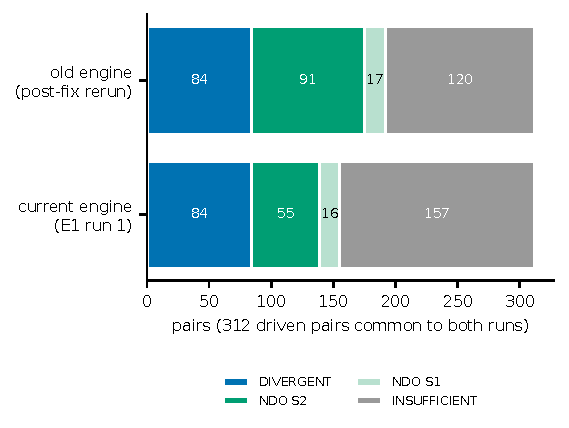
\includegraphics[width=\columnwidth]{../../results/v7b_phase2_summary/figures/fig_p2_verdict_dist.pdf}
\caption{V7-B verdict distribution on the 312 driven pairs: earlier engine (post-fix rerun) versus current engine (E1 run 1). Source: \path{results/v7b_phase2_summary/p2_e1_20261118_074906/e1_analysis.json}.}\label{fig:verdictdist}
\end{figure}

\subsection{E3: detection, false assurance and abstention}
Table~\ref{tab:datasets} gives the data and Table~\ref{tab:byarm} the V7-B verdict per arm (84 \DIV{}, 157 \INS{}, 16 \NDO{}/S1, 55 \NDO{}/S2, 9 not driven). Table~\ref{tab:metrics} and Fig.~\ref{fig:metrics} give the system metrics on the 258 labelled pairs. V7-B returns \NDO{} on 13 of 106 divergent-labelled pairs (0.123) against 24 of 106 for B1 (0.226) and B1+rep (identical; 0 discordant pairs), and detects 75 of 106 (0.708) against 82 of 106 (0.774). V7-B abstains on 122 of 258 pairs (0.473; 18 divergent-labelled and 104 no-difference-labelled) and raises no false alarm on the 152 no-difference-labelled pairs, whereas B1 reports a difference on 46 of 152 (0.303). The edit-size heuristic B4 has no usable signal (1 of 106 detected).
\begin{table}[t]\centering\scriptsize\setlength{\tabcolsep}{3pt}
\caption{E3 system metrics on the 258 labelled pairs (106 divergent, 152 no-difference); 95\% project-cluster bootstrap CI ($B=10000$, seed 42). Exploratory; non-pristine data. Abstention for V7-B counts INSUFFICIENT on both truth classes (122 = 18 + 104). Source: \path{results/v7b_phase2_summary/p2_e3_20261118_092700/statistics/system_metrics.csv}.}\label{tab:metrics}
\resizebox{\linewidth}{!}{%
\begin{tabular}{lllll}
\hline
System & False assurance & Detection & Abstention & False alarm \\
\hline
B1 & 24/106 = 0.226 [0.119, 0.392] & 82/106 = 0.774 [0.609, 0.881] & 0/258 & 46/152 = 0.303 \\
B1+rep & 24/106 = 0.226 [0.120, 0.390] & 82/106 = 0.774 [0.610, 0.880] & 0/258 & 46/152 = 0.303 \\
B3 & 20/106 = 0.189 [0.097, 0.337] & 86/106 = 0.811 [0.662, 0.904] & 0/258 & 47/152 = 0.309 \\
B4 & 105/106 = 0.991 [0.981, 1.000] & 1/106 = 0.009 [0.000, 0.019] & 0/258 & 1/152 = 0.007 \\
V7-B & 13/106 = 0.123 [0.054, 0.236] & 75/106 = 0.708 [0.545, 0.816] & 122/258 = 0.473 [0.353, 0.524] & 0/152 = 0.000 \\
\hline
\end{tabular}}
\end{table}

\begin{figure*}[t]\centering
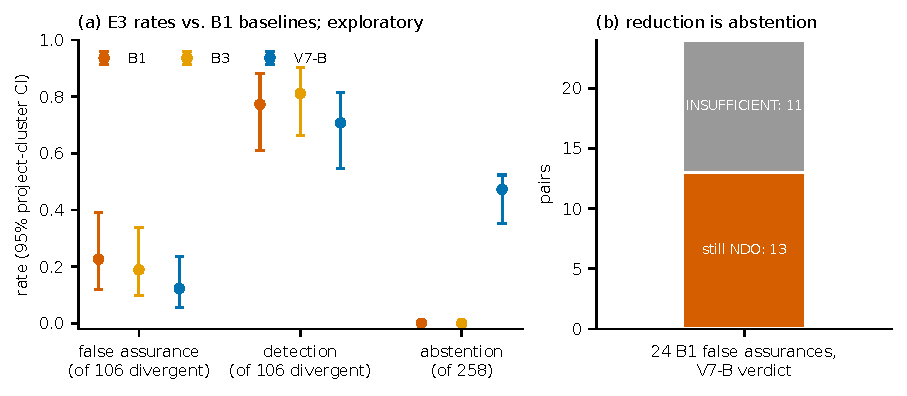
\includegraphics[width=0.85\textwidth]{../../results/v7b_phase2_summary/figures/fig_p2_metrics_vs_b1.pdf}
\caption{(a) Rates with 95\% project-cluster intervals for B1, B3 and V7-B. (b) The verdict of V7-B on the 24 pairs that B1 wrongly passes. Source: \path{results/v7b_phase2_summary/p2_e3_20261118_092700/statistics/system_metrics.csv} and \path{.../processed/dev_pairs_per_system.csv}.}\label{fig:metrics}
\end{figure*}

\textbf{Paired comparison.} Table~\ref{tab:paired} compares V7-B with B1 on the 106 divergent pairs. The false-assurance difference is $-10.4$ points (95\% CI $[-20.5,-4.3]$; 0 V7-B-only versus 11 B1-only discordant pairs; sign-flip $p=0.0010$, exact McNemar $p=0.0010$, Holm $p=0.0059$). \textbf{The +10 point rule is not met} (the improvement's lower confidence bound is 4.3 points), so the defensible wording is ``reduced by about 10 points, not shown to reach 10''. Detection is $-6.6$ points ($[-11.5,-2.6]$; 0 versus 7; sign-flip $p=0.031$; Holm $p=0.156$): a possible loss, not significant after correction and not an established harm. B3 versus B1 is not significant (sign-flip $p=0.125$, Holm 0.5). Neither the intervals nor the $p$-values license a generalisation (Section~\ref{sec:stats}).
\begin{table}[t]\centering\scriptsize\setlength{\tabcolsep}{3pt}
\caption{Paired comparisons against B1 (difference in rate, test minus reference, with 95\% project-cluster CI; test-only/ref-only discordant pairs; project-level sign-flip, exact McNemar, Holm over 4 comparisons $\times$ 2 primary outcomes). Descriptive: pairs cluster by project, data are non-pristine. The +10pp rule is not met in any row. Source: \path{results/v7b_phase2_summary/p2_e3_20261118_092700/statistics/paired_comparisons.csv}.}\label{tab:paired}
\resizebox{\linewidth}{!}{%
\begin{tabular}{llrrrrrr}
\hline
Comparison & Outcome & Diff. [CI] & b/c & Sign-flip p & McNemar p & Holm p & +10pp \\
\hline
V7-B vs B1 & false assurance & -0.104 [-0.205, -0.043] & 0/11 & 0.0010 & 0.0010 & 0.0059 & no \\
V7-B vs B1 & detection & -0.066 [-0.115, -0.026] & 0/7 & 0.0312 & 0.0156 & 0.1562 & no \\
V7-B vs B1 & abstention & +0.473 [+0.354, +0.523] & 122/0 & <1e-4 & <1e-4 & 0.0003 & no \\
V7-B vs B1 & false alarm & -0.303 [-0.352, -0.145] & 0/46 & <1e-4 & <1e-4 & 0.0002 & no \\
B3 vs B1 & false assurance & -0.038 [-0.090, -0.007] & 0/4 & 0.1250 & 0.1250 & 0.5000 & no \\
B3 vs B1 & detection & +0.038 [+0.007, +0.090] & 4/0 & 0.1250 & 0.1250 & 0.5000 & no \\
B1+rep vs B1 & detection & +0.000 [+0.000, +0.000] & 0/0 & 1.0000 & 1.0000 & 1.0000 & no \\
\hline
\end{tabular}}
\end{table}


\textbf{The reduction is entirely abstention.} Of the 24 divergent pairs that B1 (and B1+rep) wrongly pass, V7-B returns \INS{} for 11 and \NDO{} for 13 and detects none of them (Fig.~\ref{fig:metrics}b); the pre-registered attribution statistic is 11 of 11 recovered cases being \INS{} (the cluster-bootstrap interval is degenerate at $[1,1]$ because all 11 are \INS{}, and with $n=11$ it is not a precise estimate). On the 88 divergent pairs where V7-B does not abstain, V7-B detects 75 and misses 13, and B1 detects the same 75 and misses the same 13. V7-B's advantage on false assurance is therefore calibrated abstention, not extra detection. The derived, not executed, gate counterfactual (Table~\ref{tab:gate}) shows the same: relabelling every \INS{} as \NDO{} raises false assurance from 13 to 31 of 106 (0.293), and relabelling only the gate-attributable reasons gives 24 of 106 (0.226), equal to B1.
\begin{table}[t]\centering\scriptsize\setlength{\tabcolsep}{3pt}
\caption{Derived (not executed) gate counterfactual on the E3 verdicts. Source: \path{results/v7b_phase2_summary/p2_consolidated_20261118_190644/consolidated.json}, key \texttt{gate\_counterfactual\_E3}.}\label{tab:gate}
\resizebox{\linewidth}{!}{%
\begin{tabular}{lrrr}
\hline
Variant & False assurance & Rate & Abstained \\
\hline
actual V7-B & 13/106 & 0.123 & 122 \\
all INSUFFICIENT relabelled NDO & 31/106 & 0.292 & 0 \\
only gate-attributable reasons relabelled & 24/106 & 0.226 & 96 \\
\hline
\end{tabular}}
\end{table}


\textbf{Risk--coverage.} Table~\ref{tab:riskcov} and Fig.~\ref{fig:riskcov} show that V7-B decides 136 of 258 pairs (coverage 0.527; the 0.096 figure is 13/136 and mixes 75 detections with 61 \NDO{} verdicts, so it is not the error rate of \NDO{}: 13 of 61 \NDO{} verdicts are wrong versus 24 of 130 for B1) at any level, and 120 of 258 (coverage 0.465, risk 0.067) when \NDO{} requires S2; B1 decides all pairs at risk 0.271. The S3 row (coverage 0.291, 75 decided, risk 0) contains only witnessed divergences, because S3 is refused by configuration. The curve is descriptive: risk is against generator labels, baselines have no sufficiency level, and matched-coverage superiority was not computed.
\begin{table}[t]\centering\scriptsize\setlength{\tabcolsep}{3pt}
\caption{Risk--coverage (decided verdicts only; risk = errors/decided against generator or test-oracle labels). The V7-B S3 row contains only witnessed divergences because S3 is refused by configuration and no NO\_DIVERGENCE\_OBSERVED is issued at that level. Source: \path{results/v7b_phase2_summary/p2_e3_20261118_092700/statistics/risk_coverage.csv}.}\label{tab:riskcov}
\resizebox{\linewidth}{!}{%
\begin{tabular}{llrrr}
\hline
System & Min. level for NDO & Coverage & Risk [CI] & Decided \\
\hline
B1 & none & 1.000 & 0.271 [0.210, 0.331] & 258/258 \\
V7-B & none & 0.527 & 0.096 [0.038, 0.212] & 136/258 \\
V7-B & S1 & 0.527 & 0.096 [0.039, 0.210] & 136/258 \\
V7-B & S2 & 0.465 & 0.067 [0.023, 0.167] & 120/258 \\
V7-B & S3 & 0.291 & 0.000 [0.000, 0.000] & 75/258 \\
\hline
\end{tabular}}
\end{table}

\begin{figure}[t]\centering
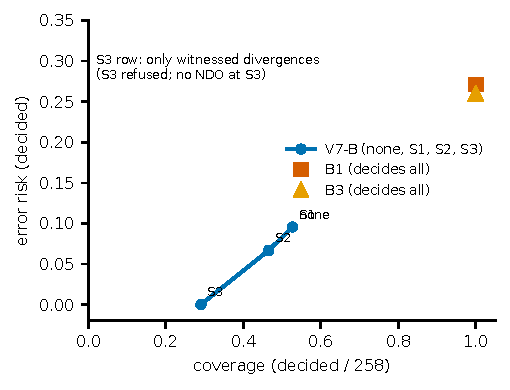
\includegraphics[width=\columnwidth]{../../results/v7b_phase2_summary/figures/fig_p2_risk_coverage.pdf}
\caption{Coverage versus error risk (descriptive; generator and test-oracle labels). Source: \path{results/v7b_phase2_summary/p2_e3_20261118_092700/statistics/risk_coverage.csv}.}\label{fig:riskcov}
\end{figure}

\textbf{Change relative to the earlier post-fix run.} Detection (0.708) and false assurance (0.123) are unchanged and baselines are identical, but abstention rose from 0.360 to 0.473 because 54 pairs now return \INS{}(\texttt{unmodelled\_change}) (Table~\ref{tab:reasons}). This is the conservative rule A-U1, which is unrefined; part of the increase may be noise of that rule, and only three of the affected pairs were inspected. It is not shown that the shift reduced false assurance.
\begin{table}[t]\centering\scriptsize\setlength{\tabcolsep}{3pt}
\caption{Primary reason of the INSUFFICIENT verdicts in the E3 run (312 driven pairs; 9 pairs are not driven). Source: \path{results/v7b_phase2_summary/p2_e3_20261118_092700/processed/k1_spike_per_pair.jsonl}.}\label{tab:reasons}
\resizebox{\linewidth}{!}{%
\begin{tabular}{lrl}
\hline
Primary reason & Pairs & Meaning \\
\hline
unmodelled\_change & 54 & changed lines without executable code (rule A-U1) \\
unsupported\_signature & 49 & renamed entry or unsupported signature \\
changed\_region\_not\_activated & 40 & no input reached the changed lines \\
unobservable\_outcome & 8 & lossy or degenerate observation \\
resource\_limit & 4 & limit hit on a side or both \\
nondeterministic & 1 & a version is not self-consistent \\
import\_error & 1 & import or entry failure \\
total & 157 &  \\
\hline
\end{tabular}}
\end{table}

\begin{table}[t]\centering\scriptsize\setlength{\tabcolsep}{3pt}
\caption{V7-B verdict per arm, E3 run (321 pairs). Source: \path{results/v7b_phase2_summary/p2_e3_20261118_092700/processed/dev_pairs_per_system.csv}.}\label{tab:byarm}
\resizebox{\linewidth}{!}{%
\begin{tabular}{lrrrrr}
\hline
Arm & DIV & INSUF. & NDO S1 & NDO S2 & Not driven \\
\hline
bugsinpy\_units & 6 & 32 & 0 & 8 & 9 \\
quixbugs\_buggy\_fixed & 27 & 4 & 0 & 0 & 0 \\
quixbugs\_sp\_negatives & 1 & 60 & 3 & 21 & 0 \\
synthetic\_equivalent & 1 & 45 & 8 & 18 & 0 \\
synthetic\_changed & 49 & 16 & 5 & 8 & 0 \\
total & 84 & 157 & 16 & 55 & 9 \\
\hline
\end{tabular}}
\end{table}


\subsection{E4--E6: ablation, S2 floor and runtime}
The results of E4 and E5 are in Section~\ref{sec:ablation} and those of E6 in Section~\ref{sec:runtime}.

\subsection{E7: verification and corruption suite}
\texttt{python -m sbgv7 verify} returned exit 0 for all 828 evidence directories (E3 and E1, run 1 and run 2), covering \DIV{}, \NDO{}/S1, \NDO{}/S2 and \INS{} with every reason code produced. On copies, the corruption suite behaved as pre-registered in 42 of 42 runs (Table~\ref{tab:e7}): a flipped byte, truncation, a deleted record, a missing package, a broken chain, an edited \texttt{verdict.json}, a deleted log (exit 2) and a simulated size-cap omission (exit 4) are detected, and a modification without re-chaining is detected. The documented limitations behave as predicted and are \emph{not} detected: a writer who edits unverified fields (run timings, run status or detail) and recomputes the chain and \texttt{log\_head} produces a log that verifies, and a deleted \texttt{verdict.json} is not detected. \texttt{verify} recomputes recorded facts and executes nothing, so it cannot detect a lie in a recorded observation. 828 of 828 verified is therefore consistency of the records, not validation of the system and not tamper-proofing.
\begin{table}[t]\centering\scriptsize\setlength{\tabcolsep}{3pt}
\caption{E7 corruption suite: 14 corruption cases applied to copies of three evidence directories each (one per verdict class), 42 runs. Exit codes of \texttt{verify}: 0 verified, 1 mismatch, 2 unreadable or missing, 4 evidence omitted by size cap. ``As expected'' means as pre-registered; cases ending with exit 0 are documented limitations that the check does not detect. Source: \path{results/v7b_phase2_summary/p2_e7_20261118_190612/corruption_results.json}.}\label{tab:e7}
\resizebox{\linewidth}{!}{%
\begin{tabular}{lrrrl}
\hline
Case & Runs & Exit code & As expected & Outcome \\
\hline
flip\_byte\_in\_record & 3 & 1 & yes & detected \\
truncate\_drop\_last\_record & 3 & 1 & yes & detected \\
truncate\_mid\_line & 3 & 1 & yes & detected \\
delete\_middle\_record & 3 & 1 & yes & detected \\
remove\_package\_rechained & 3 & 1 & yes & detected \\
break\_chain\_prev & 3 & 1 & yes & detected \\
verdict\_json\_changed & 3 & 1 & yes & detected \\
verdict\_json\_log\_head\_changed & 3 & 1 & yes & detected \\
evidence\_missing & 3 & 2 & yes & detected \\
source\_omitted\_rechained & 3 & 4 & yes & detected \\
forge\_meta\_timing\_rechained & 3 & 0 & yes & NOT detected (documented limit) \\
forge\_run\_status\_rechained & 3 & 0 & yes & NOT detected (documented limit) \\
forge\_without\_rechain & 3 & 1 & yes & detected \\
delete\_verdict\_json & 3 & 0 & yes & NOT detected (documented limit) \\
\hline
\end{tabular}}
\end{table}

